\documentclass{article}
\usepackage{graphicx}
\usepackage[utf8]{inputenc}
\usepackage{fullpage}
\usepackage[linesnumbered,ruled,vlined]{algorithm2e}
\usepackage{enumitem}
\usepackage{url}
\usepackage{amsmath}
\usepackage{gensymb}
\usepackage{float}

\parindent0in
\pagestyle{plain}
\thispagestyle{plain}

\newcommand{\assignment}{Homework 1}
\newcommand{\duedate}{March 13, 2020}

% \renewcommand\thesubsection{\arabic{subsection}}

\title{Homework 1}
\author{João Pedro de Abreu Marciano}
\date{}

\begin{document}

Fundação Getulio Vargas\hfill\\
Estruturas de Dados e Algoritmos\hfill\textbf{\assignment}\\
Prof.\ Jorge Poco\hfill\textbf{Due:}: \duedate\\
\smallskip\hrule\bigskip

{\let\newpage\relax\maketitle}
\maketitle


\section{Induction [3pts]}
Answers should be written in this document. 

\begin{enumerate}
  \item Prove by Induction that:
  \( \sum_{i=1}^{n}i^2=\frac{n(n+1)(2n+1)}{6} \qquad\forall n \geq 0\)
    \\
    \\
    Case $n=0$: \\
    $0 = \frac{0(0+1)(0\cdot 2+1)}{6}$, which is clearly true.
    \\
    \\
    Suppose that $\sum_{i=1}^{k} i^2 = \frac{k(k+1)(2k+1)}{6}$. We want to prove for $n=k+1$. So,
    \begin{equation*}
    \begin{split}
        \sum_{i=1}^{k+1} i^2 &= \sum_{i=1}^{k} i^2 + (k+1)^2 \\
         & = \frac{k(k+1)(2k+1)}{6} + (k+1)^2 \\
         & = (k+1)(\frac{k(2k+1)}{6} + (k+1)) \\
         & = (k+1)\frac{2k^2+k+6k+6}{6} \\
         & = (k+1)\frac{2k^2+7k+6}{6} \\
         & = (k+1)\frac{(k+2)(2k+3)}{6} \\
         & = \frac{(k+1)(k+2)(2k+3)}{6} \\ 
         & = \frac{(k+1)((k+1)+1)(2(k+1)+1)}{6} 
    \end{split}
    \end{equation*}
    
    Thus, by induction, \( \sum_{i=1}^{n}i^2=\frac{n(n+1)(2n+1)}{6} \qquad\forall n \geq 0\)
    \\
  \item Prove by Induction that:
  $\forall n \geq 7$ it is true $3^n<n!$
  \\
  \\
  Case $n=7$: \\
  $3^7 = 2187 < 5040 = 7!$
  \\
  \\
  Suppose that $3^k=k!$. We want to prove for $n=k+1$.
  \begin{equation*}
    \begin{split}
        3^{k+1} & = 3\cdot 3^k \\
        & < 3\cdot k! \\
        & < (k+1)!
    \end{split}
  \end{equation*}
  
  Thus, by induction, $\forall n \geq 7$ it is true $3^n<n!$.
  \\
  
  \item Prove by Induction that $\forall n \geq 0$
  \[
    \left \lceil\frac{n}{2} \right \rceil=
    \left\{
    \begin{array}{ll}
    \frac{n}{2}& \textrm{if $n$ is even}\\
    \frac{n+1}{2}& \textrm{if $n$ is odd}
    \end{array}
    \right.
  \]
  
  Case $n=0$: \\
  \[ \left \lceil\frac{0}{2} \right \rceil = \frac{0}{2}\]
  \\
  Case $n=1$: \\
  \[ \left \lceil\frac{1}{2} \right \rceil = \frac{1+1}{2}\]
  \\
  \\
  Suppose that \(
        \left \lceil\frac{k}{2} \right \rceil=
        \left\{
        \begin{array}{ll}
        \frac{k}{2}& \textrm{if $k$ is even}\\
        \frac{k+1}{2}& \textrm{if $k$ s odd}
        \end{array}
        \right.
    \). We want to prove for $n=k+2$ in the cases that $k$ is even and $k$ is odd. \\
    
  Case $k$ is even: \\
  \begin{equation*}
    \begin{split}
        \left \lceil\frac{k+2}{2} \right \rceil & = \left \lceil\frac{k}{2} \right \rceil + 1 \\
        & = \frac{k}{2} + 1 \\
        & = \frac{k+2}{2}
    \end{split}
  \end{equation*}
  
  Case $k$ is odd: \\
  \begin{equation*}
    \begin{split}
        \left \lceil\frac{k+2}{2} \right \rceil & = \left \lceil\frac{k}{2} \right \rceil + 1 \\
        & = \frac{k+1}{2} + 1 \\
        & = \frac{(k+2)+1}{2}
    \end{split}
  \end{equation*}
  \\
  Thus, by induction in the evens and in the odds, $\forall n \geq 0$
  \(
    \left \lceil\frac{n}{2} \right \rceil=
    \left\{
    \begin{array}{ll}
    \frac{n}{2}& \textrm{if $n$ is even}\\
    \frac{n+1}{2}& \textrm{if $n$ is odd}
    \end{array}
    \right.
  \).
  \\
  
  \item Prove by induction that a number is divisible by 3 if and only if the sum of its digits is divisible by 3.
  \\
  \\
  Lemma: 
  $$10^n\equiv 1 \pmod{3} \hspace{20pt} \forall n\geq0$$
  
  Proof by induction of the lemma:
  
  Case n=0: $10^0\equiv 1 \pmod{3}$.
  
  Suppose that for $n=k$, $10^k\equiv 1 \pmod{3}$. So, 
  
  \begin{equation*}
    \begin{split}
        10^{k+1} &\equiv 10\cdot10^k \pmod{3} \\
        &\equiv 10\cdot 1 \pmod{3} \\
        &\equiv 10 \pmod{3} \\
        &\equiv 1 \pmod{3}
    \end{split}
  \end{equation*}
    
  By induction, the lemma is true.
    
  Proving ($\Rightarrow$): 
  
  Given a number $n$ divisible by 3 and let $S(n)$ be the sum of the digits of $n$. $n$ can be written as $n = \sum_{i=0}^k 10^i a_i$, where the $a_i$ is the ($i+1$)-th digit of $n$ counting from right to left.
  So, 
  
  \begin{equation*}
    \begin{split}
        n &\equiv \sum_{i=0}^k 10^i a_i \pmod{3} \\
        &\equiv \sum_{i=0}^k a_i \pmod{3} \\
        &\equiv S(n) \pmod{3}
    \end{split}
  \end{equation*}
  
  As we wanted to prove.
  
  
  Proving ($\Leftarrow$): 
  
  Given a number $n$ where $S(n)$ divisible by 3. So,
  
  \begin{equation*}
    \begin{split}
        S(n) &\equiv \sum_{i=0}^k a_i \pmod{3} \\
        &\equiv \sum_{i=0}^k 10^i a_i \pmod{3} \\
        &\equiv n \pmod{3}
    \end{split}
  \end{equation*}
  
  As we wanted to prove.
  
  \item Prove that any integer greater than 59 can be formed using only 7 and 11 cent coins.
  
  Case $n=60$: $11\cdot 1 + 7\cdot 7 = 60$
  
  Case $n=61$: $11\cdot 3 + 7\cdot 4 = 61$
  
  Case $n=62$: $11\cdot 5 + 7\cdot 1 = 62$
  
  Case $n=63$: $11\cdot 0 + 7\cdot 9 = 63$
  
  Case $n=64$: $11\cdot 2 + 7\cdot 6 = 64$
  
  Case $n=65$: $11\cdot 4 + 7\cdot 3 = 65$
  
  Case $n=66$: $11\cdot 6 + 7\cdot 0 = 66$
  \\
  \\
  Suppose that it is valid for $k-7$. We want to prove for $n=k$.
  
  Using the hypothesis, there are $x_0$ and $y_0$ such that
  \begin{equation*}
    \begin{split}
        & 11\cdot x_0 + 7\cdot y_0 = k-7 \\
        & 11\cdot x_0 + 7\cdot (y_0+1) = k \\
    \end{split}
  \end{equation*}
  
  So there are integers $x_1 = x_0$ and $y_1 = y_0+1$ such that $11\cdot x_1 + 7\cdot y_1 = k$.
  
  Thus, by induction, any integer greater than 59 can be formed using only 7 and 11 cent coins.
  \\
  
  \item Prove by induction that $F_{n+k}=F_{k}F_{n+1}+F_{k-1}F_{n}$.
  
  
  We have that $F_0 = 0$, $F_1 = 1$ and $F_2 = 1$.
  
  Case n=1:
  \begin{equation}
    \begin{split}
        F_{k+1}=F_{k}F_{2}+F_{k-1}F_{1}=F_{k}+F_{k-1} \hspace{10pt} \forall k \geq1 \\
    \end{split}
  \end{equation}
  which is the definition of the Fibonacci sequence.
  
  Suppose that $F_{n+k}=F_{k}F_{n+1}+F_{k-1}F_{n}$, $\forall k\geq 1$. We want to prove for $n+1$.
  Switching $k$ for $k+1$:
  
  \begin{equation*}
    \begin{split}
        F_{n+k+1} & = F_{k+1}F_{n+1}+F_{k}F_{n} \\
        \text{Using property $(1)$: } F_{n+k+1} & = (F_{k}+F_{k-1})F_{n+1}+F_{k}F_{n} \\
        F_{n+k+1} & = F_{k}(F_{n+1}+F_{n}) + F_{k-1}F_{n+1}  \\
        F_{(n+1)+k} & = F_{k}F_{(n+1)+1} + F_{k-1}F_{(n+1)}  \\
    \end{split}
  \end{equation*}
  
  Thus, by induction, $F_{n+k}=F_{k}F_{n+1}+F_{k-1}F_{n} \hspace{40pt} \forall k\geq 1 \hspace{5pt} \forall n\geq 0$.
  \\
  
  \item Prove by induction in $n$ that \(\sum_{m=0}^{n}{n \choose m}=2^n\).
  
  Case n=0:
  \begin{equation*}
    \begin{split}
        \sum_{m=0}^{0}{n \choose m} = {0 \choose 0} = 1 = 2^0 \\
    \end{split}
  \end{equation*}
  
  Lemma: 
  \[ {n \choose m} + {n \choose m+1} = {n+1 \choose m+1}  \hspace{20pt} \forall n,m \geq 0 \]
  \\
  
  Suppose that \(\sum_{m=0}^{n}{n \choose m}=2^n\). We want to prove for $n+1$. So, using the lemma,
  
  \begin{equation*}
    \begin{split}
        \sum_{m=0}^{n+1}{n+1 \choose m} &= \sum_{m=0}^{n-1}({n \choose m} + {n \choose m+1}) + {n+1 \choose 0} + {n+1 \choose n+1} \\
        &= \sum_{m=0}^{n-1}({n \choose m} + {n \choose m+1}) + {n \choose 0} + {n \choose n} \\
        &= 2\sum_{m=0}^{n}{n \choose m} \\
        &= 2\cdot 2^n \\
        &= 2^{n+1}
    \end{split}
  \end{equation*}
  
  Thus, by induction, \(\sum_{m=0}^{n}{n \choose m}=2^n \hspace{20pt} \forall n \geq 0\).
  \\
  
  \item Prove by induction that a graph with $n$ vertices can have at most  $\dfrac{n(n-1)}{2}$ edges.
  
  Case n=1 is clearly $0=\dfrac{1(1-1)}{2}$.
  
  Suppose that with $k$ vertices have at the most $\dfrac{k(k-1)}{2}$ edges. Analysing a $k+1$ graph, its maximum number of edges is the maximum number of edges of a graph with $k$ vertices plus $k$ edges (that comes from inserting a new vertex that is connected to each one of the other $k$ vertices). So, this number is $\dfrac{k(k-1)}{2}+k = \dfrac{k^2-k+2k}{2} = \dfrac{k^2+k}{2} = \dfrac{k(k+1)}{2}$.

  
  Thus, by induction, a graph with $n$ vertices can have at most  $\dfrac{n(n-1)}{2}$ edges.
  \\
  
  \item Prove by induction that a full binary tree\footnote{\url{http://web.cecs.pdx.edu/~sheard/course/Cs163/Doc/FullvsComplete.html}} with $n$ levels has $2^n-1$ vertices.
   
  Case n=1 we have that $1 = 2^1-1$, which is trivially true.
 
  Suppose that it is valid for $n$ levels. We want to prove for $n+1$.
  If we look at the second and below levels of the tree, it is easy to see that it will have two full trees of levels-size $n$ each. So, the total amount of vertex of our tree of our tree is our root plus $2$ times the amount of vertices at a tree of $n$ levels. Then, this number is $1+2(2^n-1)=2^{n+1}-1$.
  
  
  Thus, by induction, a full binary tree with $n$ levels has $2^n-1$ vertices.
  \\
  
  
  \item A polygon is convex if each pair of points in the polygon can be joined by a straight line that does not leave the polygon. Prove by induction in $n>3$ that the sum of the angles of a polygon of $n$ vertices is $180(n-2)$.
  
  Case n=3 is a triangle, which we know that has $180\degree = (3-2)180$.
  
  
  Suppose that it is valid for a $n$-sided polygon  We want to prove for a $n+1$-sided polygon. 
  As the polygon is convex we can connect two vertices in a way that it will construct a triangle and a $n-1$-sided polygon. And the sum of the internal angles of these two polygons are equal to the sum of the internal angles of our first polygon. So, this number is 
  \[180 + (n-2)180 = (n-1)180\]
  
  Thus, by induction, the sum of the angles of a convex polygon of $n$ vertices is $180(n-2)$ $\forall n\geq 3$ .
  \\
  
  
\end{enumerate}

\section{Correctness of bubblesort [3pts]}
Bubblesort is a popular, but inefficient, sorting algorithm. It works by repeatedly swapping adjacent elements that are out of order.

\begin{algorithm}[H]
\SetAlgoLined
  \For{$i = 1$ \textbf{to} $A.length -1$} {
    \For{$j = A.length$ \textbf{downto} $i + 1$} {
      \If{$A[j] < A[j-1]$} {
        exchange $A[j]$ with $A[j-1]$
      }
    }
  }
\caption{BUBBLESORT(A)}
\end{algorithm}

\begin{enumerate}[label=\Alph*]
  \item \textbf{(0.5pt)} Let $A'$ denote the output of BUBBLESORT(A). To prove that BUBBLESORT is correct, we need to prove that it terminates and that

  \begin{equation} \label{eq:1}
    A'[1] \leq A'[2] \leq ... \leq A'[n]
  \end{equation}

  where $n = A.length$. In order to show that BUBBLESORT actually sorts, what else do we need to prove?

  \textbf{Answer:}

  We also need to prove that $A'$ has the same elements of $A$.
\\


  The next two parts will prove inequality~(\ref{eq:1}).

  \item \textbf{(1.0pt)} State precisely a loop invariant \textbf{for} the for loop in lines 2–6, and prove that this loop invariant holds. Your proof should use the structure of the loop invariant proof presented in this chapter.
  
  
  \textbf{Loop invariant:} The element $A[j-1]$ is the lowest element of the list $A[j-1:n]$ at the end of the loop.
  
  Base for induction $j=n$: the list $A[n-1,n]$ has two elements. If it doesn't enter the "if" structure it means that $A[n]>=A[n-1]$, hence $A[n-1]$ is the lowest element of $A[n-1,n]$. On the other hand, if it enters the "if" structure it means that $A[n]<A[n-1]$. And then the line $4$ changes these two elements, whence $A[n-1]<A[n]$, in other words, $A[n-1]$ is the lowest element of $A[n-1,n]$.
  
  
  Suppose that the element $A[j]$, with $j>i+1$ is the lowest element of the list $A[j:n]$. And then it returns to the beginning of the loop with $j <-> j-1$. We now look at the list $A[j-1:j]$. Using the same argument used in the base of the induction $A[j-1]$ is the lowest element of the list $A[j-1:j]$ at the end of the loop. As the $A[j]$ of $A[j:n]$ was the lowest element at the beginning of the loop, $A[j-1]$ is the lowest element of the list $A[j-1:n]$ at the end of the loop. Hence, by induction, this loop invariant is proved.
  

  \textbf{PS: I'm considering $A = A[1:n]$, as the algorithm.}


  \item \textbf{(1.0pt)} Using the termination condition of the loop invariant proved in part (B), state a loop invariant for the for loop in lines 1–7 that will allow you to prove inequality~(\ref{eq:1}). Your proof should use the structure of the loop invariant proof presented in this chapter.


  \textbf{Loop invariant:} $A[1:i+1]$ is ordered and $A[k]$ is lower than any element of $A[i+1:n]$ for all $1 \leq k \leq i$ at the end of the loop.
  
  If it is true the inequality $(2)$ is trivial, by taking $i=n-1$. So, $A[1:n-1+1] = A[1:n] = A'$ is ordered, like we wanted to prove. Beyond that, it has the same elements of $A$ in the beginning of the algorithm, as the only change made in the elements was done by an exchange at the inner loop.
  
  \textbf{Prove of the loop invariant:} 
  
  Base for induction $i=1$: When the inner loop terminates $j=i+1=2$, using its loop invariant $A[j-1]=A[1]$ is the lowest element of the list $A[1:n]$. Thus $A[1:2]$ is ordered at the end of the loop.
  
  Suppose that the loop invariant is valid for $i-1$, with $i < n-1$, so $A[1:i]$ is ordered at the end of the loop. Using the same argument as in the base, we confirm that $A[i:i+1]$ is ordered and $A[i+1]$ is the lowest element of $A[i+1:n]$. Using the hypothesis and the fact that $A[i]$ and $A[i+1]$ is greater than any of the elements of $A[1:n-1]$, we conclude that the loop invariant is true for $i$. Hence, by induction, the loop invariant is true, as we wanted to prove.


  \item \textbf{(0.5pt)} What is the worst-case running time of BUBBLESORT? How does it compare to the running time of insertion sort?
  
  \textbf{Answer:}
  
  The worst case is the descending order, as it is for the insertion sort too. It still is $O(n^2)$ in the worst case, but it takes a longer time than any other sequence to sort. That is, it has a higher constant for when it is descending in comparison to the mean complexity. Beyond that, in general, the insertion sort has a lower constant than the bubble sort, so it is faster.
  
  
\end{enumerate}


\section{Insertion Sort - Mergesort [4pts]}
Implement the insertion sort and merge sort using the template \texttt{test.py} (use Python 3.X). Create a \texttt{test.cpp} file and write the equivalent code from \texttt{test.py} in C++, ie., the functions: main, \texttt{insertion\_sort}, \texttt{merge\_sort}, and \texttt{is\_sorted}. For the random number generations you can use the \texttt{rand} function from \texttt{cstdlib}\footnote{\url{http://www.cplusplus.com/reference/cstdlib/rand/}}. Your code should print the tuple (number of objects, time insertion\_sort, time merge\_sort)

You must submit both \texttt{test.py} and \texttt{test.cpp}. Graphs and descriptions must be included in this document. 

\subsection{Random Order}
\begin{enumerate}
  \item Create 10 sets of numbers in random order. The sets must have \{10k, 20k, 30k, ..., 100k\} numbers.
  
  \item Sort these numbers using the 2 algorithms and calculate the time each algorithm takes for each set of numbers.
  
  \item Generate a plot (using excel or another tool) showing a \emph{linechart}, where the $x$-axis is the ``number of elements", and the $y$-axis is the time that the algorithms took in C++ and Python. This plot must have 6 lines of different colors with a legend.
  
  \item Write a small paragraph (3 to 4 lines) describing the results.
  
\end{enumerate}

All the graphs will be in logarithmic scale so that they give us more comparison information, which is not possible to have without it because the python insertion sort algorithm time is a lot larger than the others.


\begin{figure}[H]
  \centering
  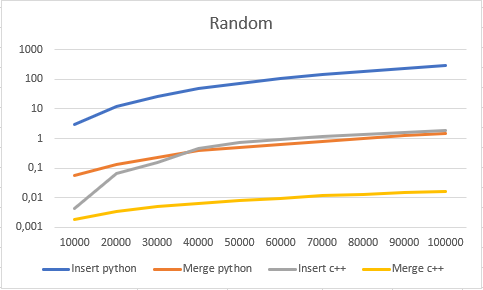
\includegraphics[width=0.7\linewidth]{Random.PNG}
  \caption{Time x Elements graph for random lists}
  \label{fig:boat1}
\end{figure}

We can see that the insertion sort takes more time to sort in both languages. The low number of elements together with the log scale don't let it highlights the difference between the complexity of the two algorithms. But the merge sort algorithm is $O(n log(n))$ while the insertion sort algorithm is $O(n^2)$ for random lists. Beyond that, we can see that the language C++ is faster, in general, than the language python; the same thing will repeat in the next cases.


\subsection{Ascending Order}
Do the same experiment when the numbers are ordered in ascending order.


\begin{figure}[H]
  \centering
  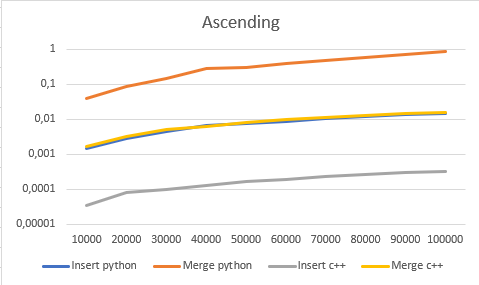
\includegraphics[width=0.7\linewidth]{Ascending.PNG}
  \caption{Time x Elements graph for ascending lists}
  \label{fig:boat1}
\end{figure}

Again it is not immediately the difference between the complexity of the two algorithms. But the merge sort algorithm is $O(n log(n))$ and the insertion sort algorithm is $O(n)$ for ascending lists. It is the better case for the insertion sort, while it doesn't change the complexity for the merge sort. Although it is faster merge sorting ascending lists than random lists because it has less comparisons to do, so the constant of the $O(n log(n))$ is lower.


\subsection{Descending Order}
Do the same experiment when the numbers are ordered in descending order.


\begin{figure}[H]
  \centering
  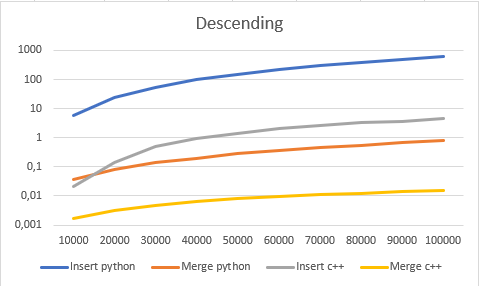
\includegraphics[width=0.7\linewidth]{Descending.PNG}
  \caption{Time x Elements graph for descending lists}
  \label{fig:boat1}
\end{figure}

In this case the insertion sort lasts considerably longer than in the case of random lists, but its complexity still is $O(n^2)$. While the complexity if the merge sort in this case stays still at $O(n log(n))$, though it terminates faster than the case of random lists for the same reason of the case ascending lists terminates faster too.

\end{document}